\section{Accesso alla piattaforma}\label{Accesso}
All'accesso della piattaforma l'utente visualizzerà la schermata principale contenente:
\begin{enumerate}
	\item Descrizione dell'azienda;
	\item Prodotti in evidenza;
	\item Barra per la ricerca dei prodotti;
	\item Icona del menù. 
\end{enumerate} 
\begin{figure}[H]
	\centering
	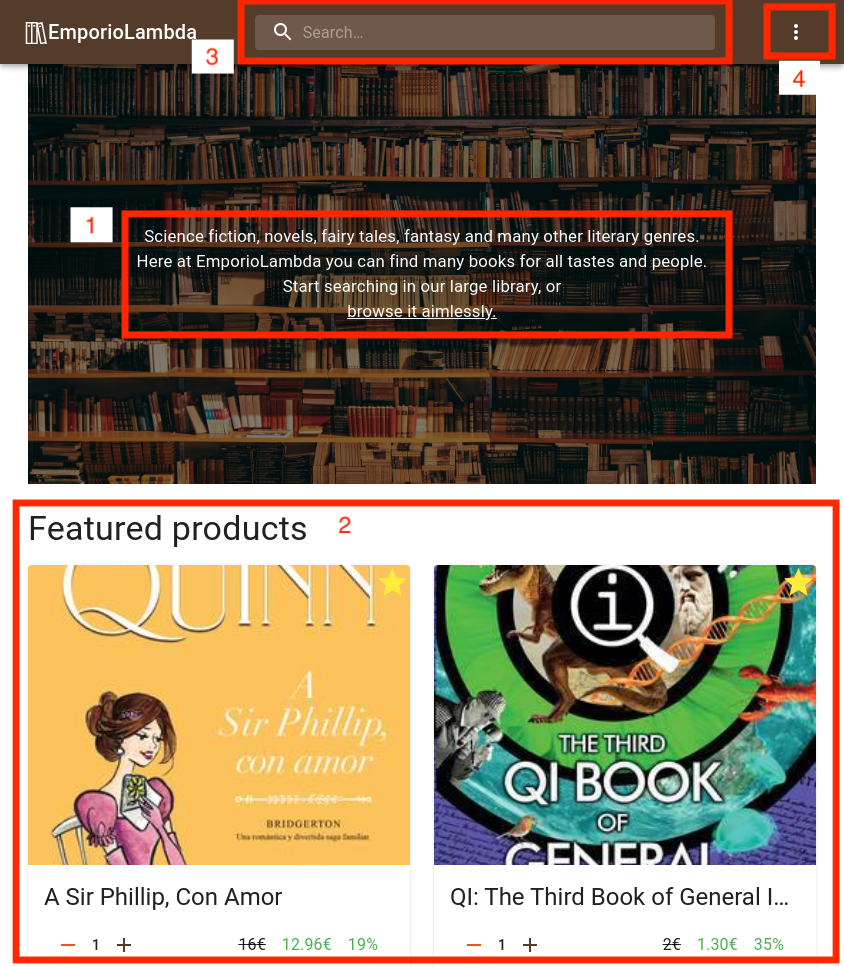
\includegraphics[scale=0.4]{Immagini/Acquirente/home_primo_accesso.png}
	\caption{Schermata principale}
	\label{fig:Home}
\end{figure}
Cliccando sull'icona del menù (4) appariranno due icone cliccabili dall'utente per poter visualizzare il proprio carrello o effettuare il login/registrazione.
\begin{figure}[H]
	\centering
	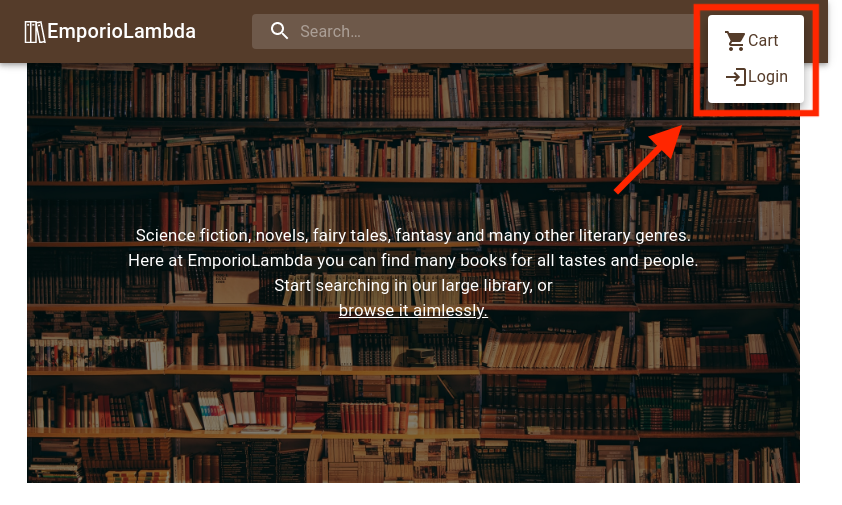
\includegraphics[scale=0.4]{Immagini/Acquirente/home-mobile-open.customer.png}
	\caption{Schermata principale con menù a tendina}
	\label{fig:Homeicone}
\end{figure}
\begin{figure}[h!]
	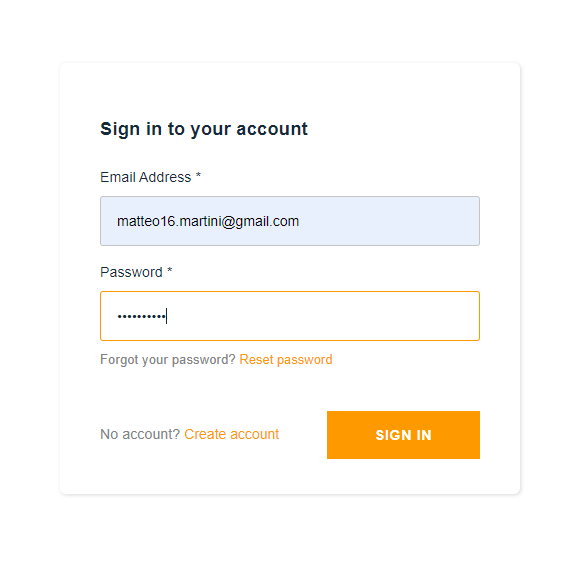
\includegraphics[scale=0.7]{Immagini/Acquirente/login.png}\quad
	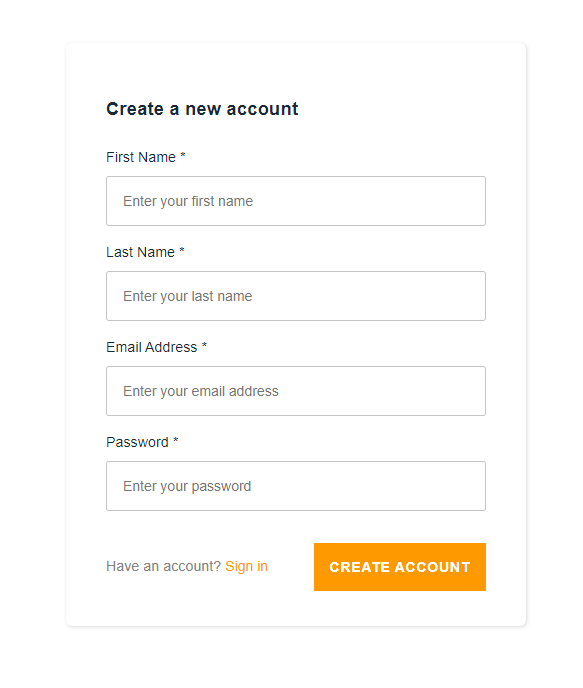
\includegraphics[scale=0.6]{Immagini/Acquirente/createAccount.png}
\end{figure}
\section{Acquirente}\label{Acquirente}
La schermata principale visualizzata comprenderà nuovamente descrizione dell'azienda, prodotti in evidenza e:
\begin{enumerate}
	\item Icona per accedere al carrello;
	\item Icona per effettuare il logout. 
\end{enumerate} 
\begin{figure}[H]
	\centering
	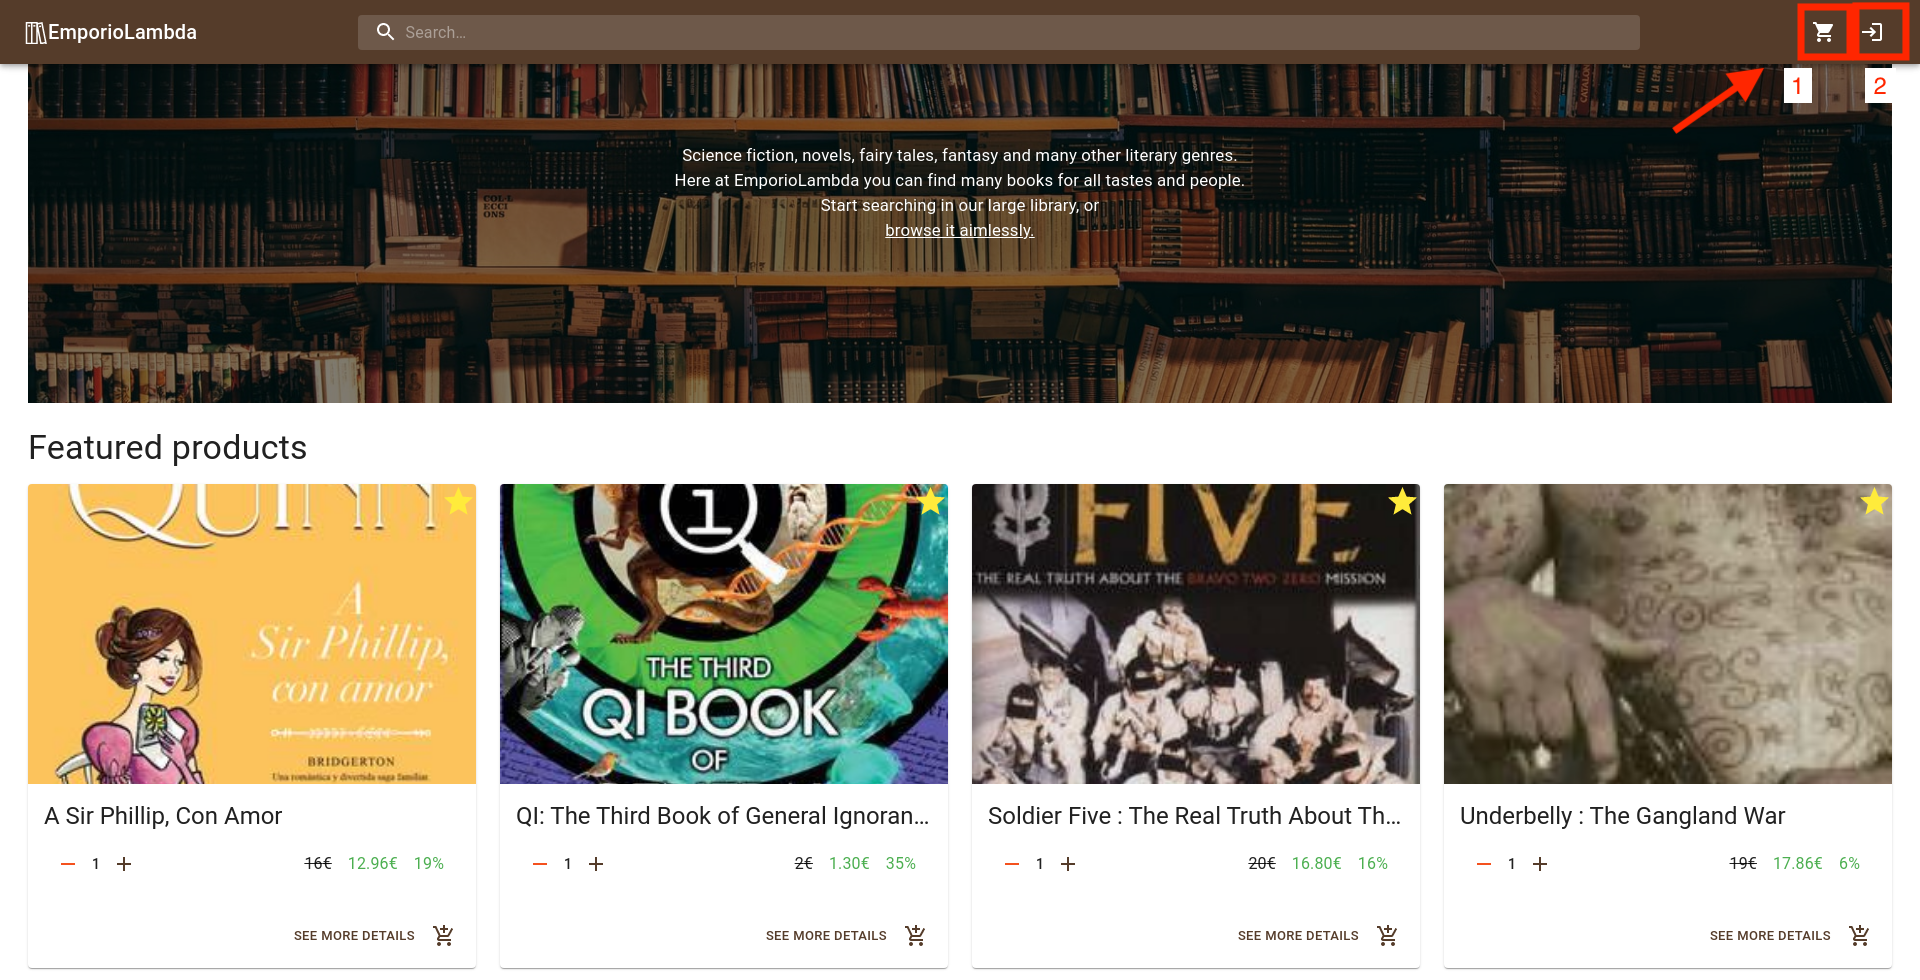
\includegraphics[scale=0.25]{Immagini/Acquirente/home.customer.png}
	\caption{Schermata principale utente autenticato}
	\label{fig:Homecustomer}
\end{figure}
\subsection{Visualizzazione specifiche di un prodotto}
L'acquirente, autenticato sulla piattaforma o come ospite, può visualizzare le specifiche di un prodotto in evidenza cliccando sullo stesso. La schermata alla quale sarà indirizzato comprenderà:
\begin{enumerate}
	\item Nome del prodotto;
	\item Elenco di immagini visualizzabili;
	\item Descrizione del prodotto;
	\item Prezzo ed eventuali sconti percentuali applicati;
	\item Categorie di appartenenza;
	\item Icone per modificare la quantità da inserire nel carrello e per inserire i prodotti nel carrello.
\end{enumerate} 
\begin{figure}[H]
	\centering
	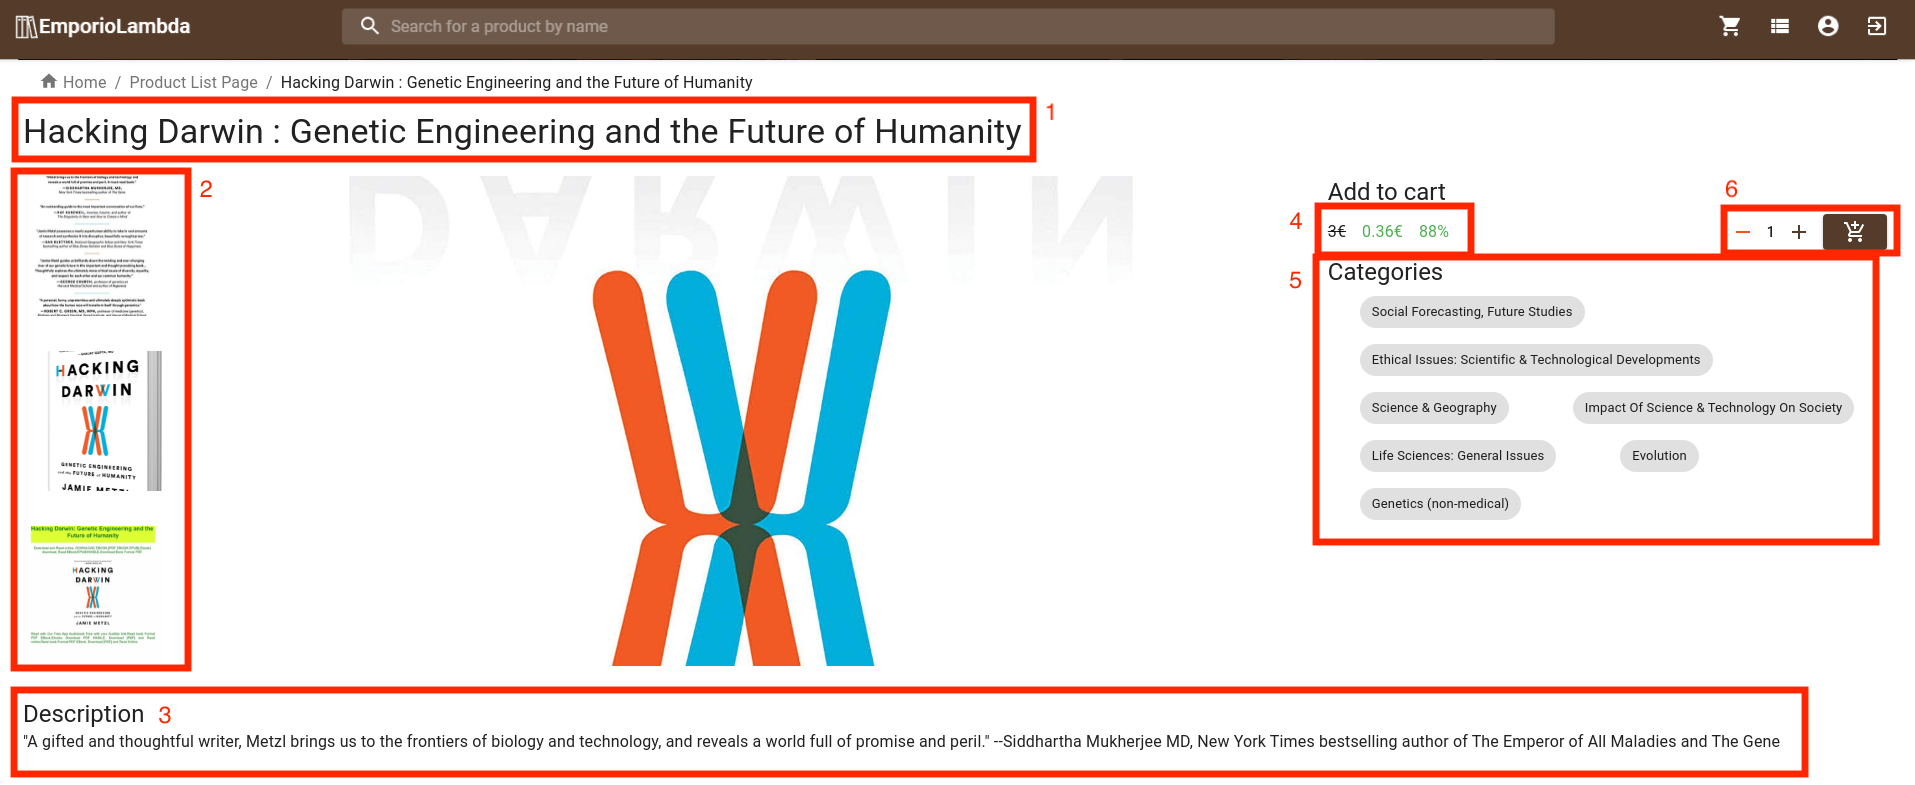
\includegraphics[scale=0.25]{Immagini/Acquirente/pdp.customer.png}
	\caption{Specifiche di un prodotto}
	\label{fig:SpecificheProdotto}
\end{figure}
\subsection{Visualizzazione elenco prodotti}
L'utente può visualizzare l'intero elenco di prodotti presenti nella piattaforma, per ognuno di essi sarà visualizzato nome, prezzo ed eventuali sconti, icone per modificare il numero di prodotti da inserire nel carrello e per inserire la quantità nel carrello. I prodotti non disponibili avranno un'indicazione sopra l'immagine del prodotto.
\begin{figure}[H]
	\centering
	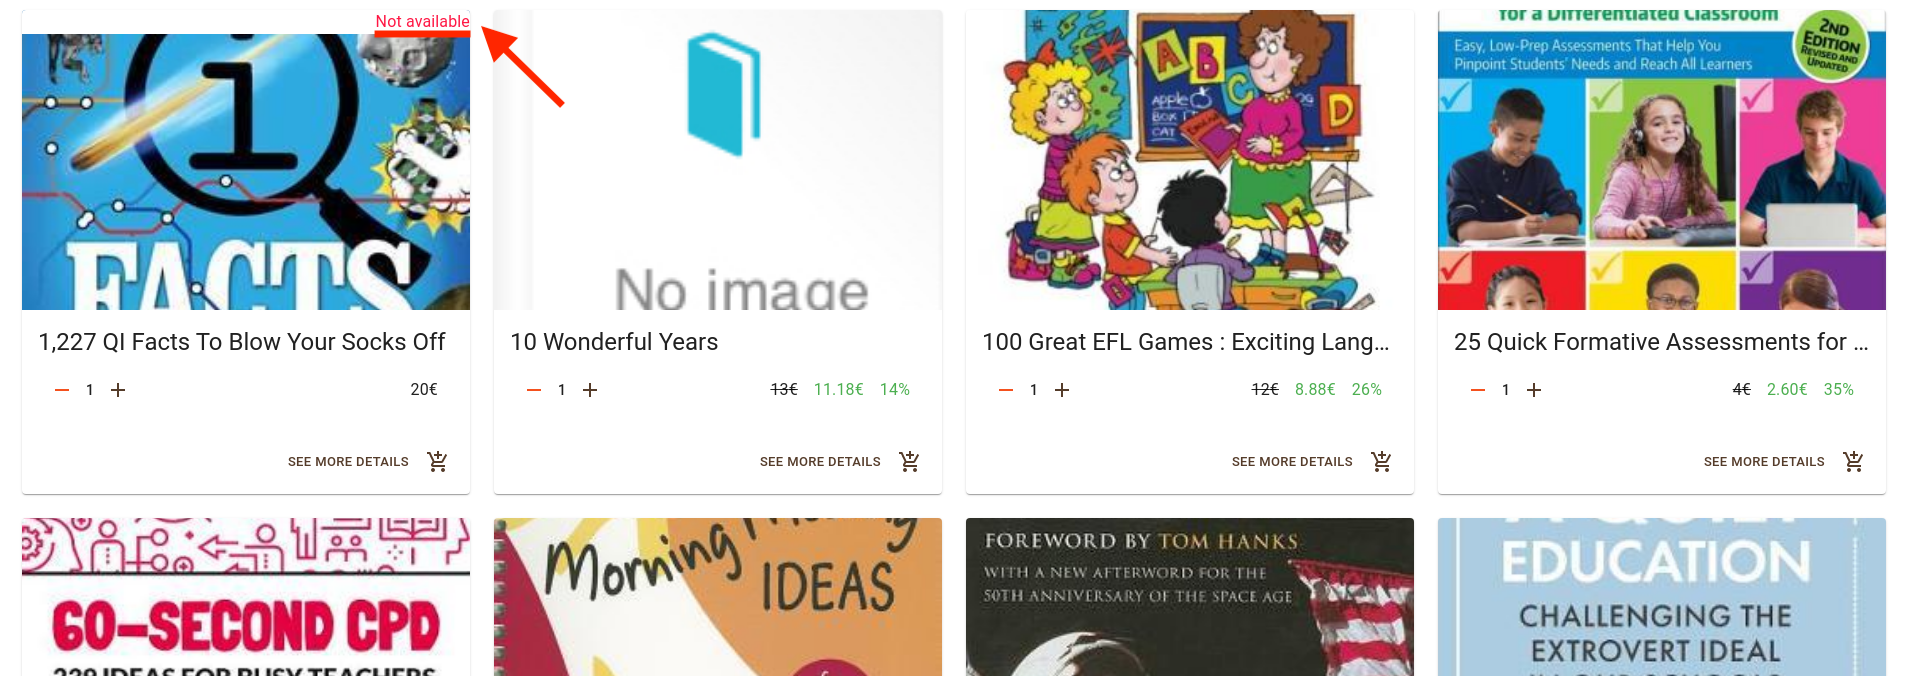
\includegraphics[scale=0.25]{Immagini/Acquirente/plp-pagination.customer.png}
	\caption{Schermata dei prodotti nella piattaforma}
	\label{fig:PLP}
\end{figure}
I prodotti possono essere visualizzati secondo un preciso ordine cliccando sull'apposita icona e selezionando il tipo di ordinamento desiderato.
\begin{figure}[H]
	\centering
	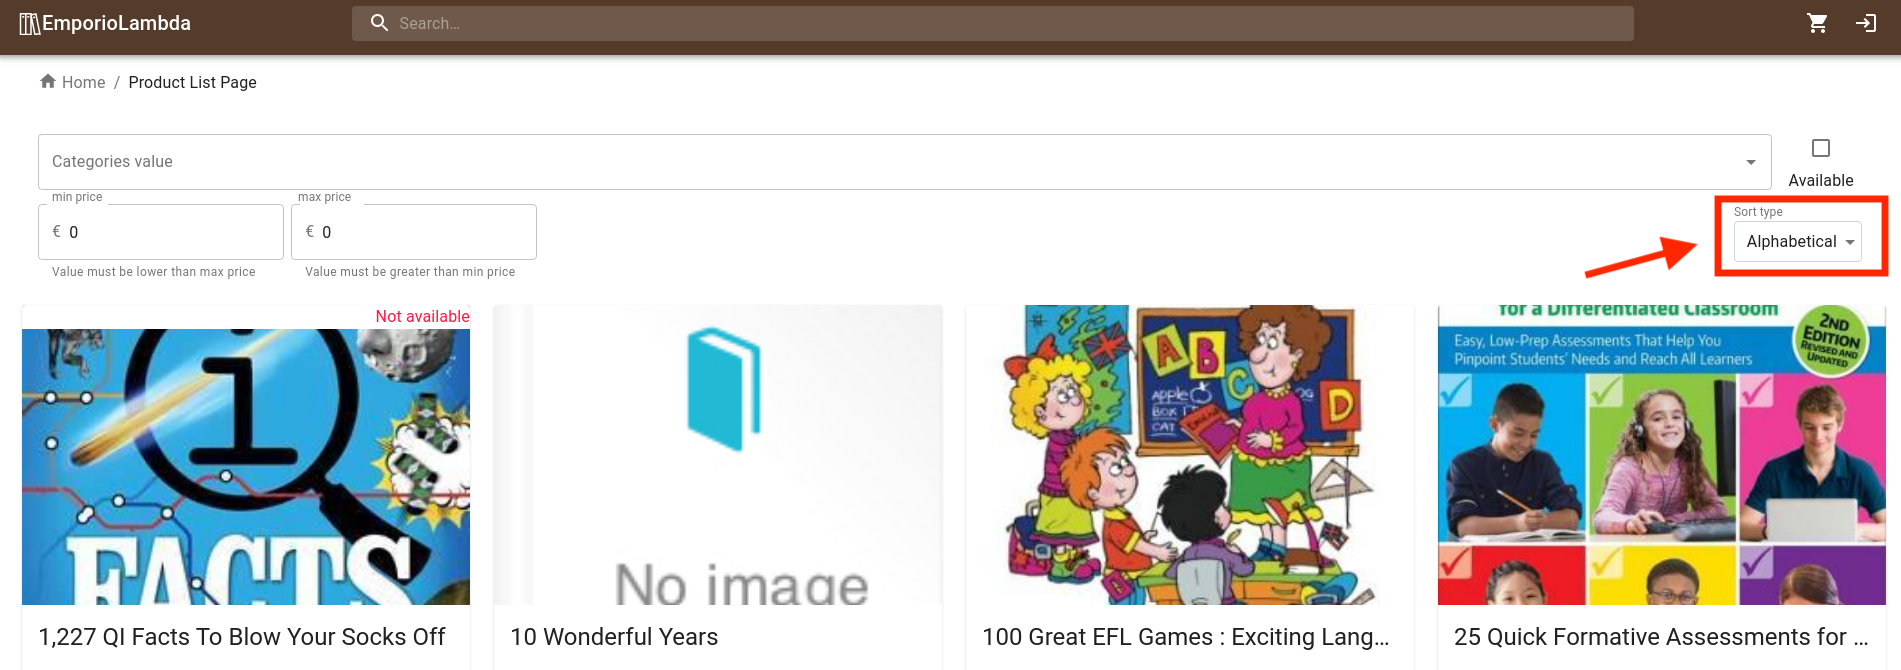
\includegraphics[scale=0.25]{Immagini/Acquirente/plp-sort1.png}
	\caption{Schermata dei prodotti nella piattaforma con ordinamento}
	\label{fig:PLPordinamento1}
\end{figure}
\begin{figure}[H]
	\centering
	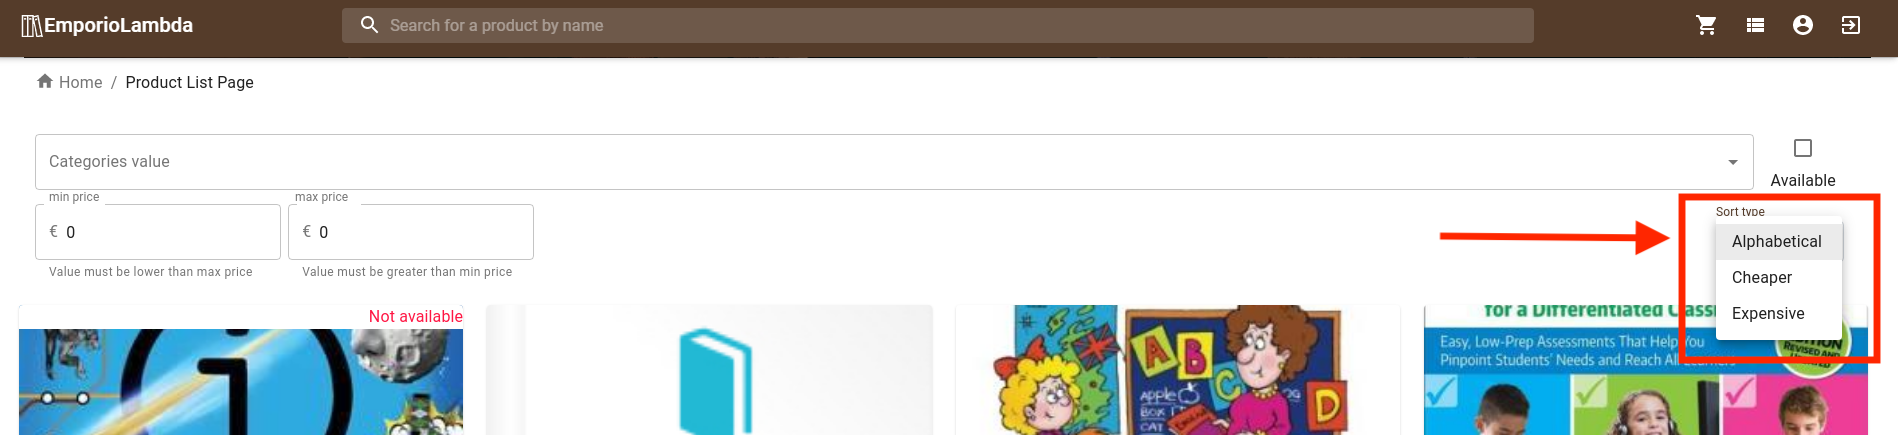
\includegraphics[scale=0.25]{Immagini/Acquirente/plp-sort-filter.png}
	\caption{Schermata dei prodotti nella piattaforma con possibili ordinamenti}
	\label{fig:PLPordinamento2}
\end{figure}
\subsection{Filtraggio dei prodotti}
Nella schermata con l'elenco prodotti l'utente può procedere a raffinare la sua ricerca impostando una serie di filtri.
\begin{figure}[H]
	\centering
	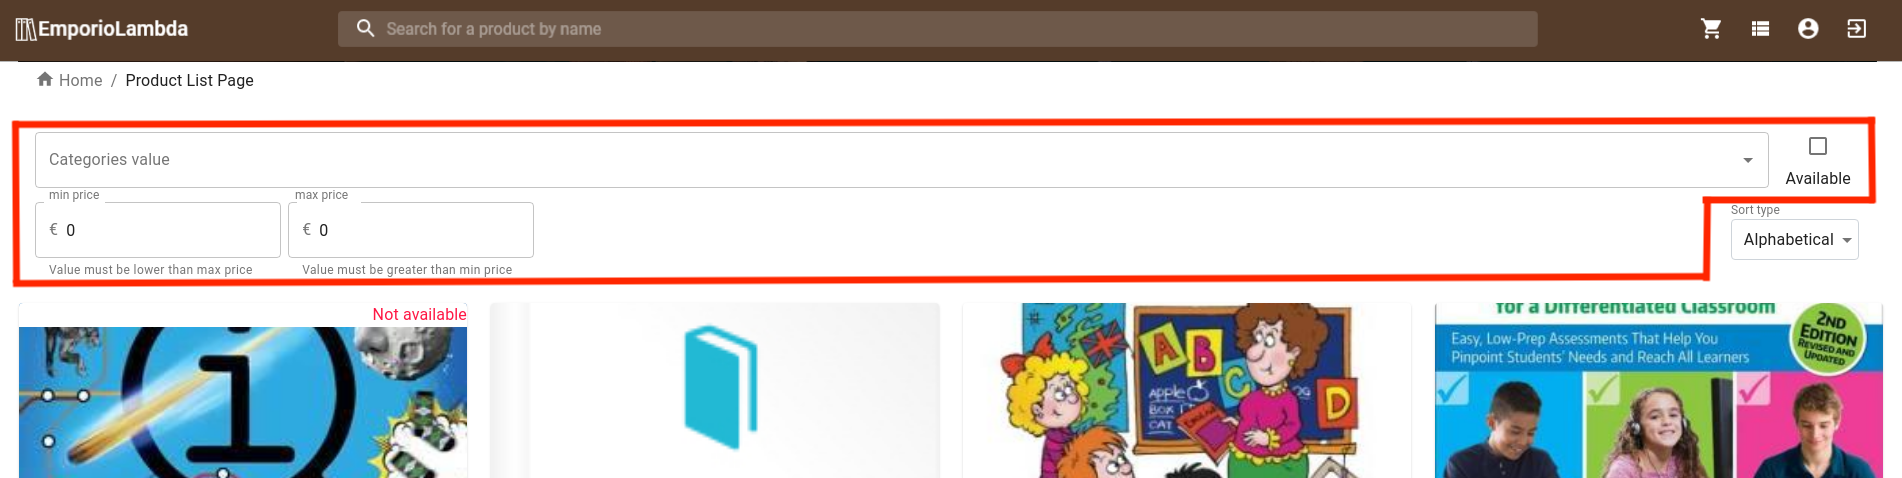
\includegraphics[scale=0.25]{Immagini/Acquirente/plp-filter.customer.png}
	\caption{Schermata dei prodotti con filtri applicabili}
	\label{fig:PLPfiltri}
\end{figure}
\subsubsection{Filtro prodotti per categorie}
Per ricercare un prodotto in base alle categorie di appartenenza, l'utente può cliccare sulla prima barra di ricerca e selezionare le categorie di interesse tra quelle visualizzate. 
\begin{figure}[H]
	\centering
	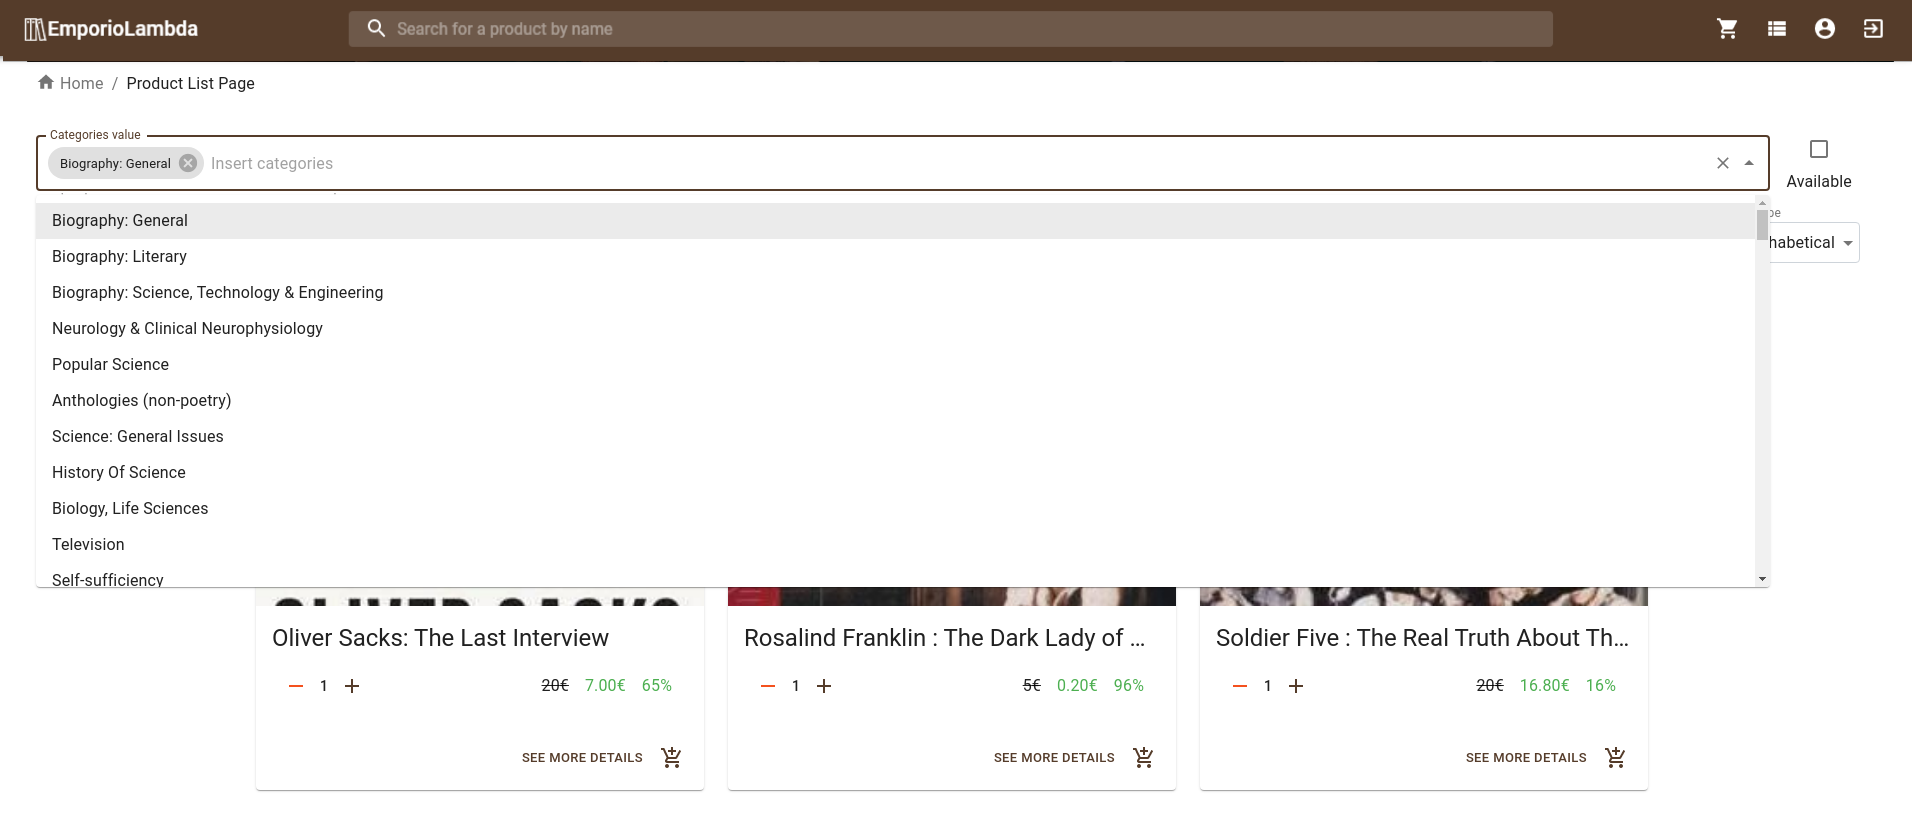
\includegraphics[scale=0.25]{Immagini/Acquirente/plp-categories-open.png}
	\caption{Filtro prodotti per categorie}
	\label{fig:PLPcategorie}
\end{figure}
\subsubsection{Filtro prodotti per disponibilità}
Per visualizzare i prodotti in base alla loro disponibilità, l'utente può selezionare la casella indicata. 
\begin{figure}[H]
	\centering
	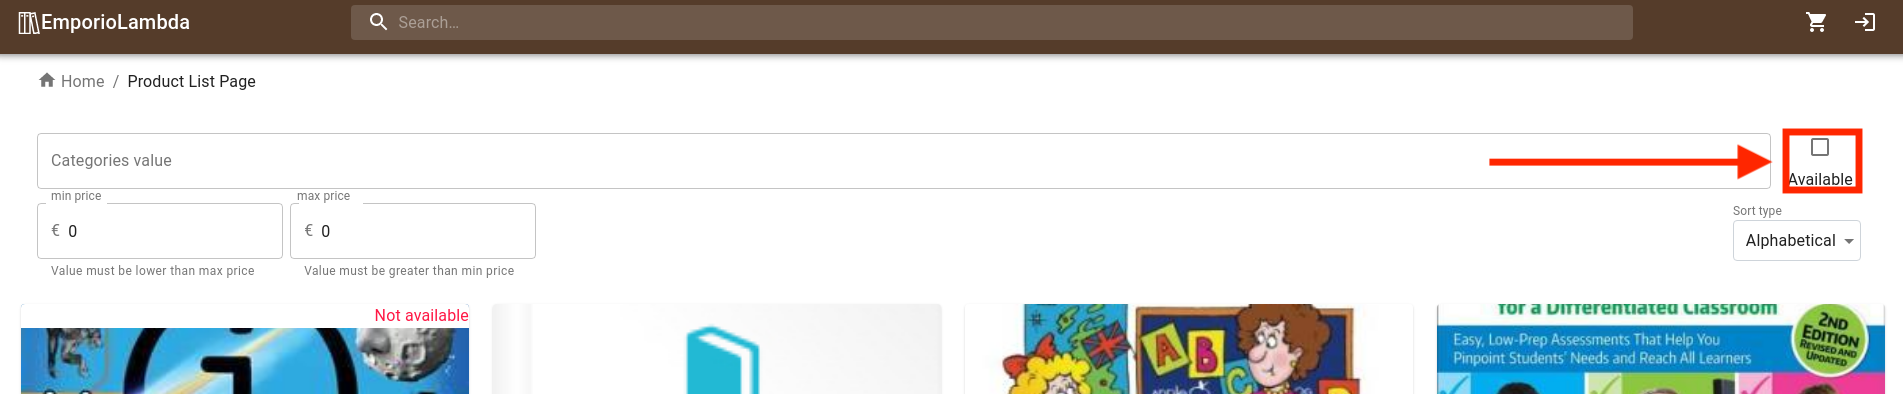
\includegraphics[scale=0.25]{Immagini/Acquirente/plp-available.png}
	\caption{Filtro prodotti per disponibilità}
	\label{fig:PLPdisponibilità}
\end{figure}
\subsubsection{Filtro prodotti per prezzo}
Per visualizzare i prodotti in base al loro prezzo, l'utente può inserire nelle caselle (1) e (2) il valore minimo e massimo per effettuare la ricerca. 
\begin{figure}[H]
	\centering
	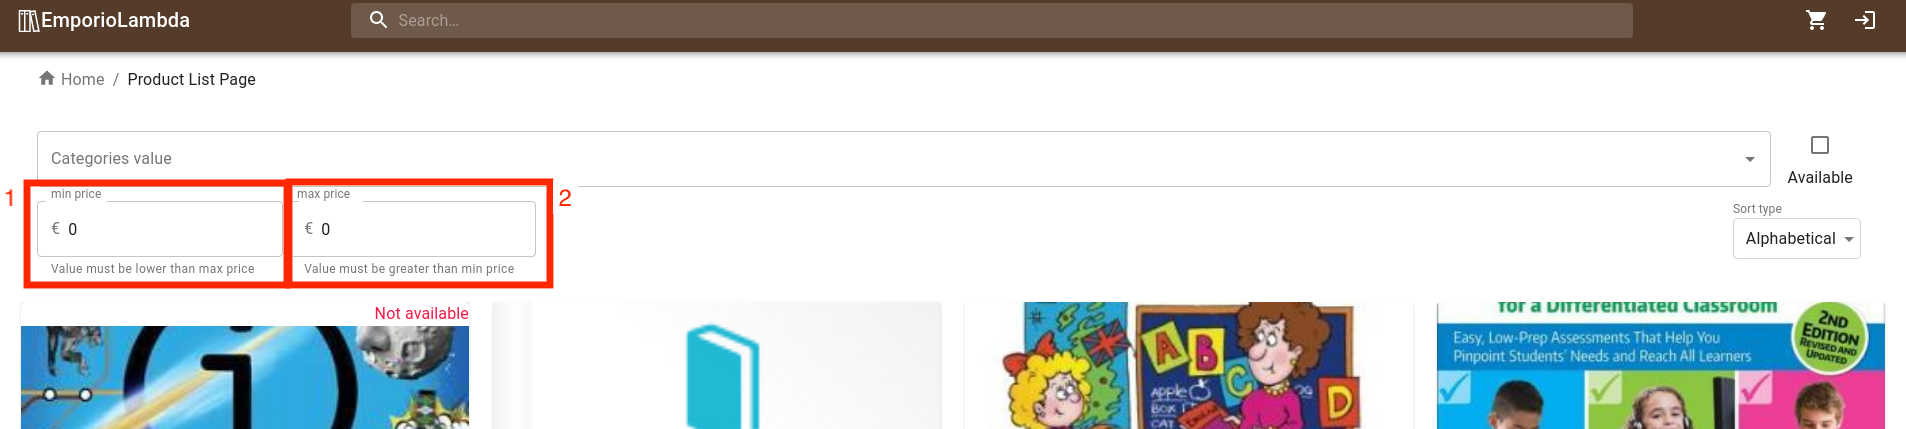
\includegraphics[scale=0.25]{Immagini/Acquirente/plp-price.png}
	\caption{Filtro prodotti per prezzo}
	\label{fig:PLPprezzo}
\end{figure}
\subsection{Visualizzazione del carrello}
Premendo sull'icona del carrello presente in ogni schermata è possibile per l'utente accedere al proprio carrello. Verranno visualizzati oltre ai vari prodotti con le loro informazioni:
\begin{enumerate}
	\item Prezzo totale;
	\item Icona per procedere al pagamento.
\end{enumerate} 
\begin{figure}[H]
	\centering
	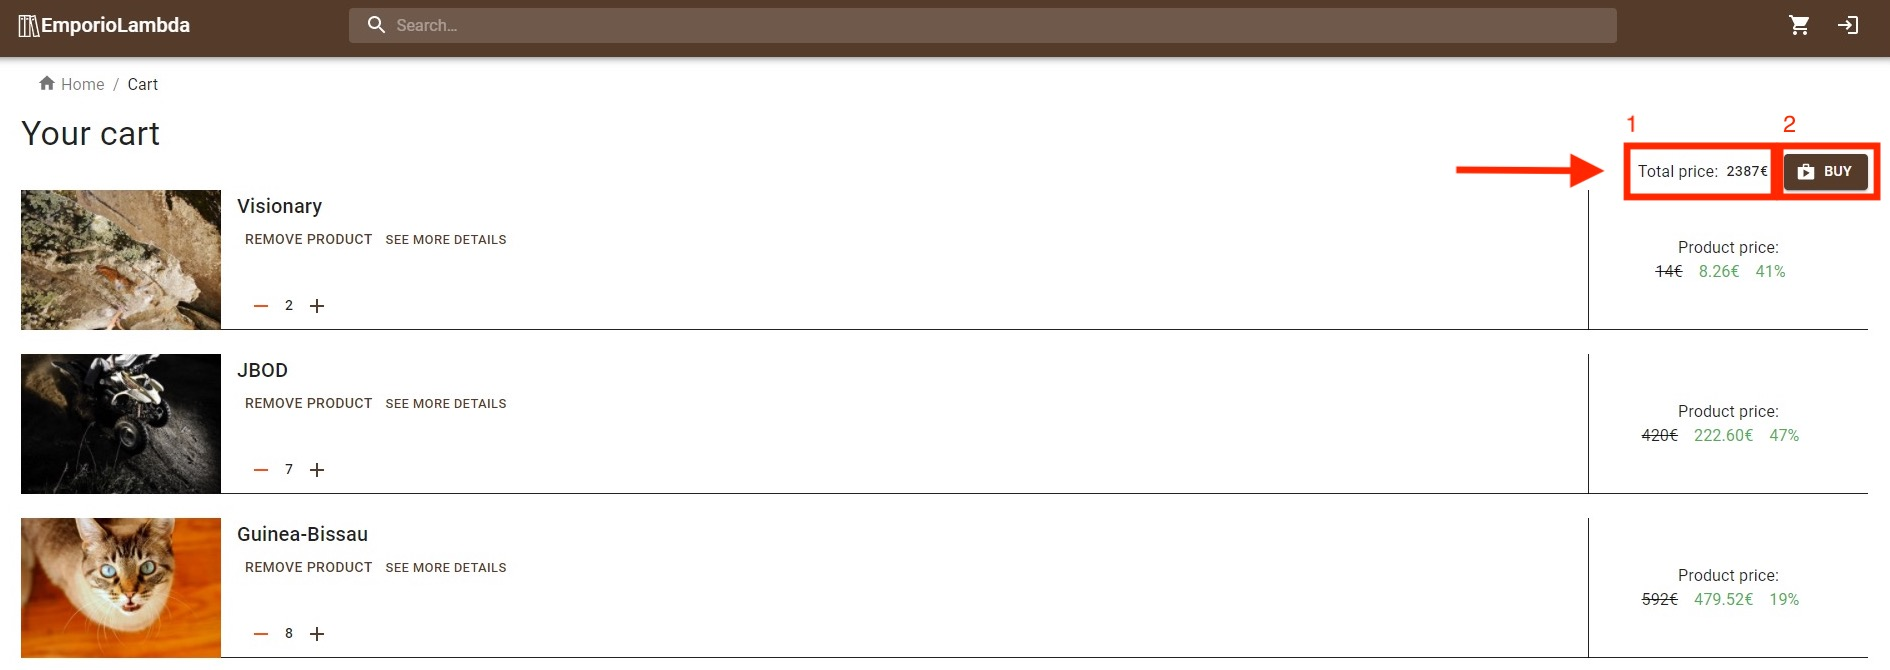
\includegraphics[scale=0.25]{Immagini/Acquirente/Cart.JPG}
	\caption{Carrello}
	\label{fig:Carrello}
\end{figure}